\newcommand{\evolvemf}{\code{evolve\_mf}}



\section{Data}


We use a wide range of data to constrain the parameters of our models. In general, we use archival
kinematic data from ground-based spectroscopy, proper motions from HST and \emph{Gaia}, number
density profiles from \emph{Gaia} supplemented with archival data, stellar mass function data from
HST photometry and pulsar timing data.

\subsection{Kinematics and density profiles}

\subsubsection{Proper motion dispersion profiles}

We use two sets of {\it Hubble Space Telescope} (HST) proper motion data. To probe the inner regions
of the cluster we use the proper motion dispersion profiles (both tangential and radial components)
from \citet{Watkins2015} which are based on a catalogue of proper motions of bright stars from
\citet{Bellini2014}. These dispersion profiles are built from stars brighter than the main sequence
turn-off (around $0.85 \ \mathrm{M}_\odot$  for 47\,Tuc). To probe the kinematics in the outer
regions of the cluster, we also use the data from \citet{Heyl2017}, for which the mean mass of the
measured stars is $0.38 \ \mathrm{M}_{\odot}$. The outer proper motion data also allows us to
constrain the amount of radial anisotropy present in the cluster, which can mimic the effect of
central dark mass in isotropic models by raising the central velocity dispersion \citep{Zocchi2017}.


\subsubsection{Line-of-sight velocity dispersion profiles}

We use the line-of-sight velocity dispersion profile from \citet{Baumgardt2018} to further constrain
the kinematics of the cluster. The dispersion profile is based on archival ESO/VLT and Keck spectra
along with previously published radial velocity data from the literature. As these radial velocity
samples are dominated by bright stars, we assume that the velocity dispersion profile traces the
kinematics of upper main-sequence and evolved stars in our models.

\subsubsection{Number density profiles}
We use the number density profile from \citet{DeBoer2019} to constrain the size and structural
parameters of the cluster. These profiles are made up of a combination of cluster members based on
Gaia DR2 data in the outer regions and surface brightness data from \citet{Trager1995} in the
central regions. The Gaia data used only includes bright stars ($m > 0.6 \ \mathrm{M}_\odot$, for
both clusters) and the literature data is dominated by bright stars, therefore in our models we
assume the profiles probe the spatial distribution of upper main sequence and evolved stars.

\subsection{Stellar mass functions}

As a constraint on the global present-day stellar mass function of the cluster, we use a compilation
of HST-based stellar mass function data from
Baumgardt\footnote{\url{https://people.smp.uq.edu.au/HolgerBaumgardt/globular/}} (2021, priv.
comm.), which represent an updated and augmented version of the stellar mass functions found in
\citet{Sollima2017}. This compilation is made up of several HST fields at varying distances from the
cluster centre. These fields extend out to $14 '$ from the cluster centre and cover a mass range of
$0.16 - 0.8 \ \mathrm{M}_\odot$. The large radial and mass ranges allow us to constrain the change
of the local stellar mass function with distance from the cluster centre and therefore the degree
mass segregation in the cluster.

\subsection{Pulsar Data}

We make use of the large population of millisecond pulsars (MSPs) in 47\,Tuc to place further
constraints on its mass distribution. We use timing solutions from \citet{Freire2017},
\citet{Ridolfi2016} and \citet{Freire2018} which include both the spin and orbital periods. We also
consider the dispersion measures of the pulsars which is a measure of how much gas the signal has
passed through on its way to the observer. When combined with internal gas models from
\citet{Abbate2018}, the dispersion measures allow us to constrain the line-of-sight position of the
pulsars within the cluster. The pulsar data is summarized in Tables \ref{tab:pulsars_spin} and
\ref{tab:pulsars_orbital}.





\section{Binary Fraction Measurements}

In order to create realistic binary populations we refer to the measurements of \citet{Milone2012}
to inform our choices of binary fraction and mass ratio distribution. For 47\,Tuc this means a flat
mass ration distribution and a binary fraction of roughly $2\%$ where the binary fraction is defined
as the ratio between binary systems and total systems (Equation \ref{eq:binary_fraction}). Because this estimate of the
binary fraction is so small, we will use it as a lower limit for the binary fraction and also test a
case where the binary fraction is around $10\%$, representing a case where the binary fraction is
significant.

\begin{equation}
    f_b = \frac{N_{bin}}{N_{bin} + N_{single}}
    \label{eq:binary_fraction}
\end{equation}


\section{Generating mass functions}

An important part of this thesis deals with generating mass functions to use as inputs to the
\code{LIMEPY} models. We do this in two main steps, we first generate a present-day mass function
comprised of only single stars, and we then modify it to include binary stars.

\subsection{Single Star Mass Functions}


To generate the mass functions comprised of single stars we use the \evolvemf{} algorithm from
\code{SSPTools}\footnote{\url{www.github.com/pjs902/ssptools}} (first presented in
\citealt{Balbinot2018}), a publicly available package for working with simple stellar populations.
As part of the previous project, we updated \evolvemf{} to include realistic prescriptions for the BH
mass function by including the effects of natal kicks in addition to dynamical ejections.

The \evolvemf{} algorithm combines precomputed grids of stellar evolution models, isochrones and
initial-final mass relations to accurately model the evolution of a given initial mass function,
including the effects of stellar evolution as well as mass loss due to escaping stars and dynamical
ejections. The algorithm returns a binned mass function at a requested evolutionary time, ideal for
use as an input in the \code{LIMEPY} models.

We parameterize the mass function as a broken power-law with breakpoints at $0.5 \ \mathrm{M}_\odot$
and $1.0 \ \mathrm{M}_\odot$. We provide to \evolvemf{} the initial mass function slopes and
breakpoints, the cluster age, metallicity and escape velocity, as well as parameters which control
the mass loss due to escaping stars and the specific binning to be used when returning the final
discrete mass-function bins. For this study we do not model the mass loss due to tidal stripping, so
we set the mass loss due to escaping stars to be zero, so we are effectively specifying the present
day mass function for low-mass stars. Figure \ref{fig:2/evolve_mf} shows the evolution of a mass
function over a span of $10 \ \mathrm{Gyr}$ (\citealt{Baumgardt2017a} found the age of 47\,Tuc to be
$11.75$ Gyr).

\begin{figure}
    \centering
    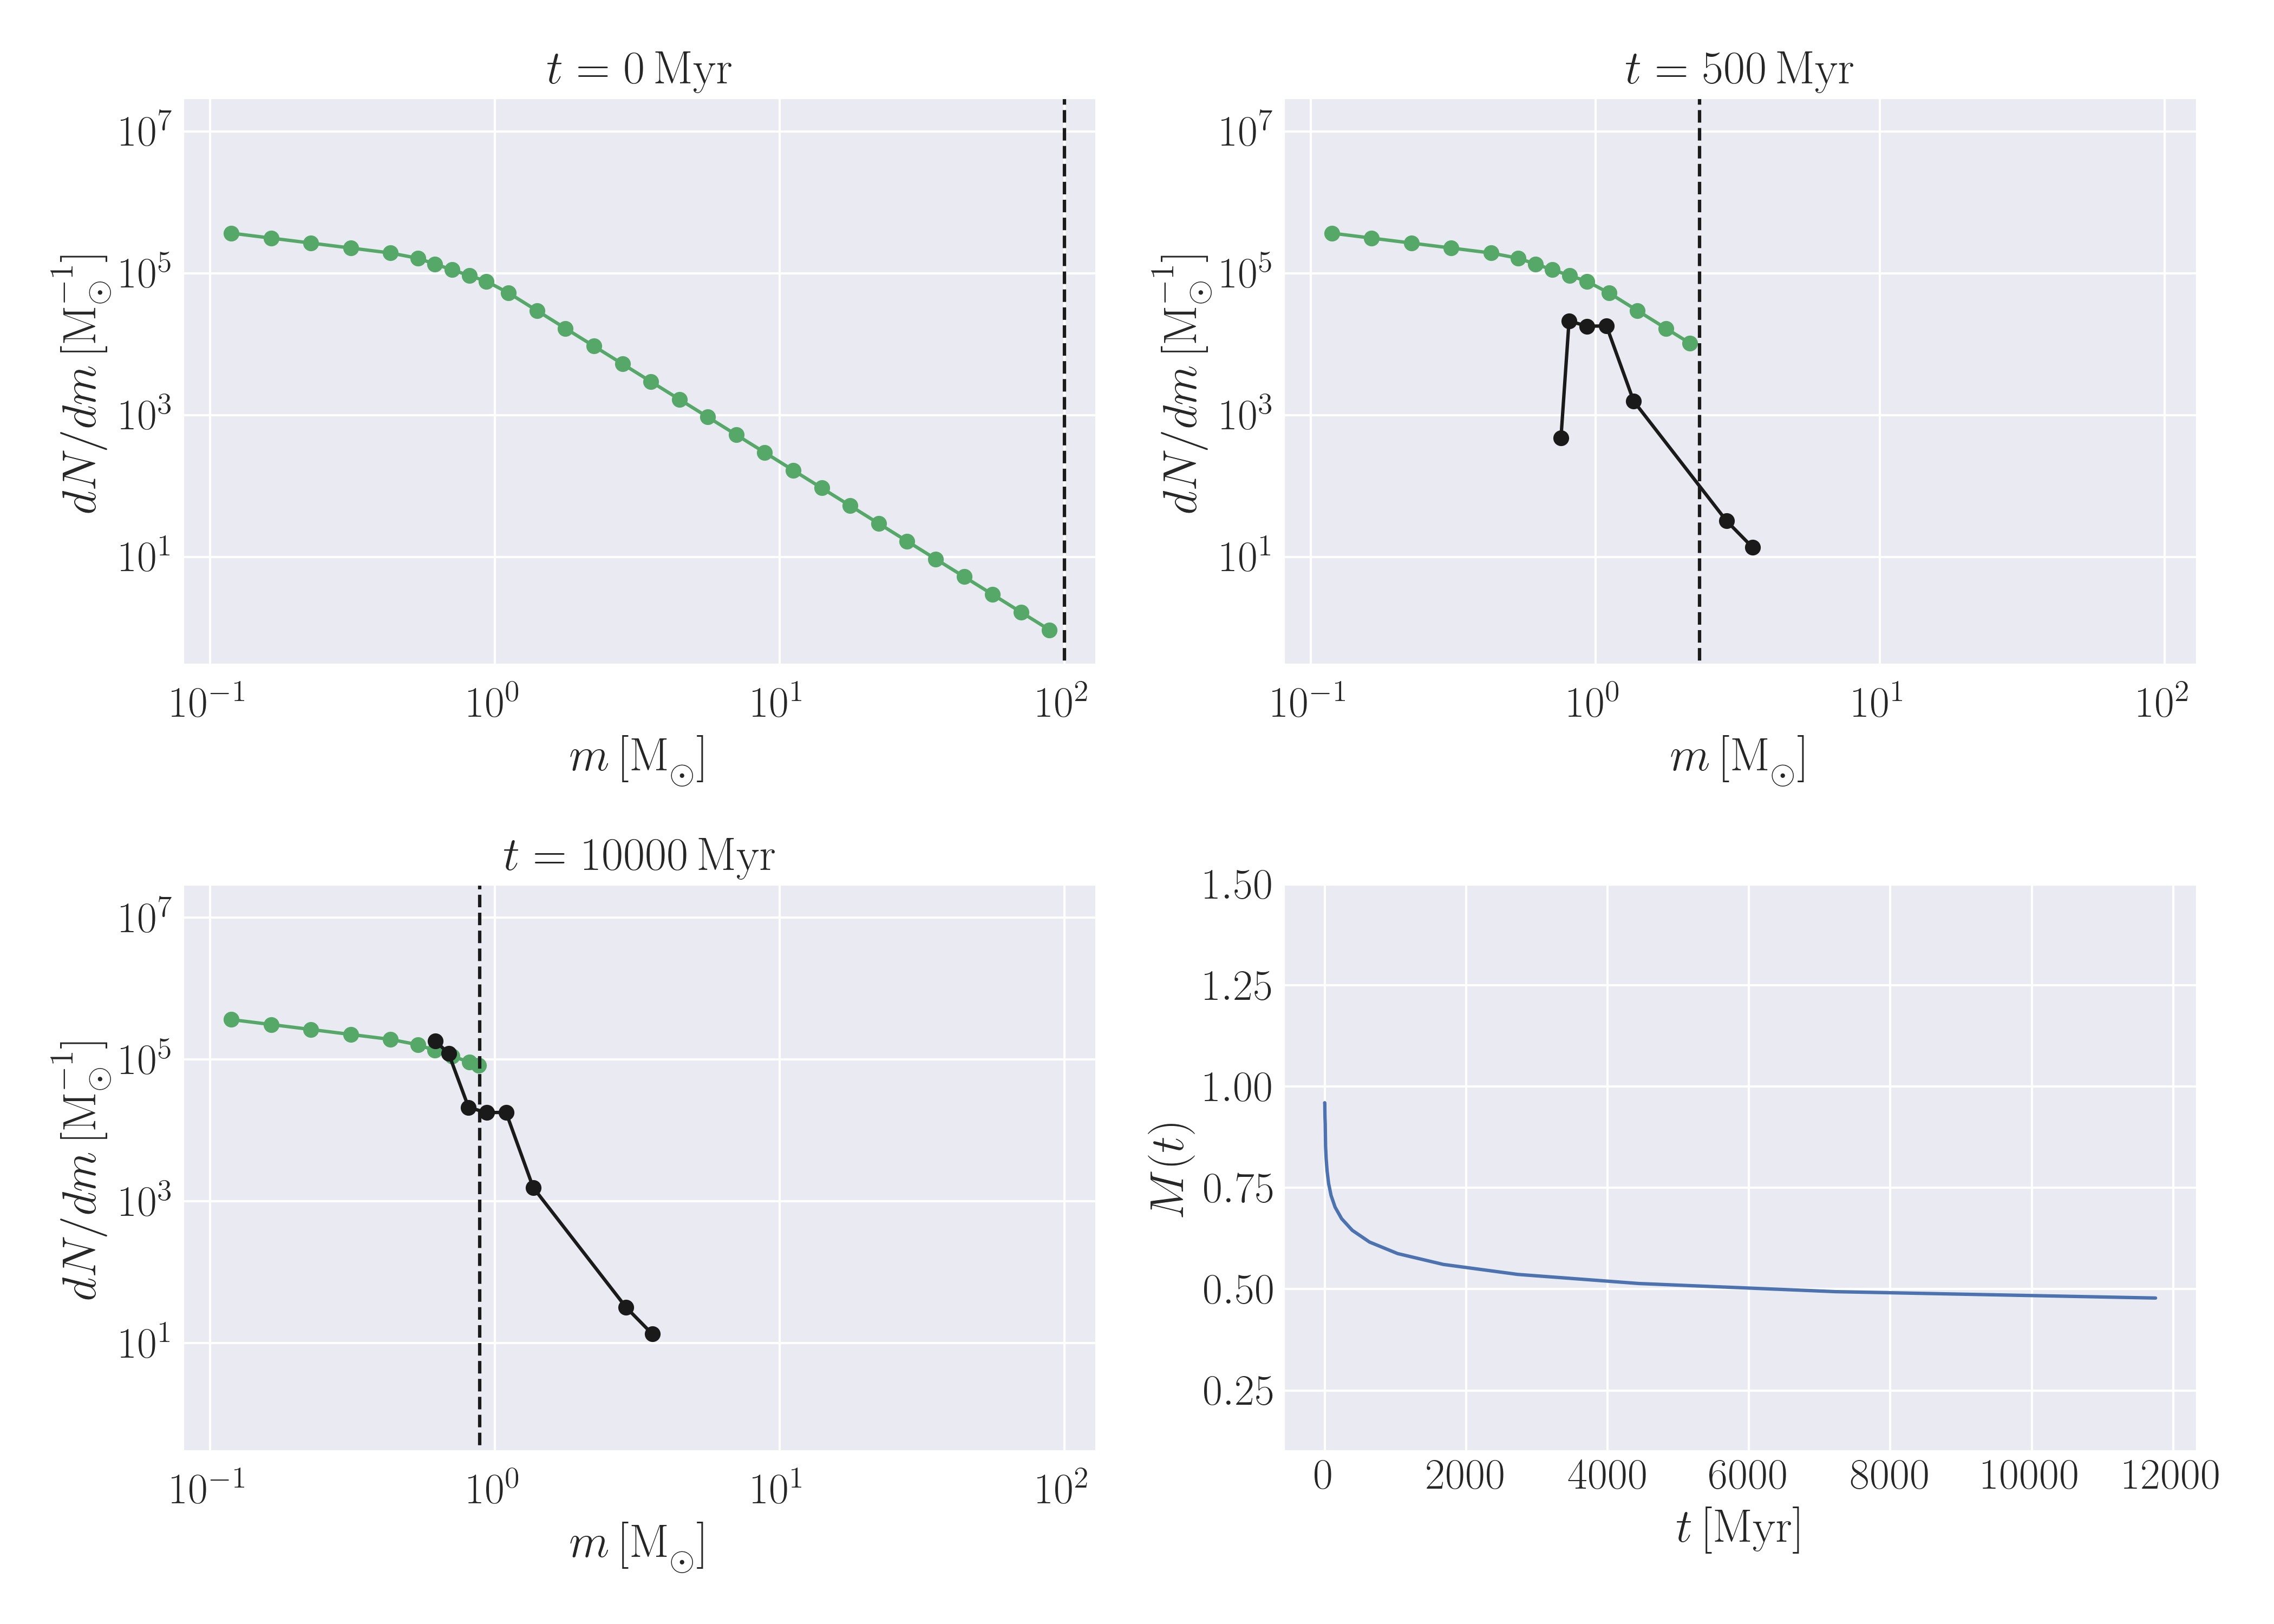
\includegraphics[width=\textwidth]{figures/evolve_mf.png}
    \caption{The evolution of a typical mass function from $t=0$ to $t=10 \ \mathrm{Gyr}$. The
        stellar bins are plotted in green while the remnant bins are plotted in black, the current
        main-sequence turn-off is plotted as a dashed black line. As the cluster ages, more and more
        main sequence stars evolve into remnants. Lower right: The evolution of the total mass of
        the cluster is plotted as a fraction of the initial mass. Mass loss is dominated by the
        effects of stellar evolution but also has contributions from ejected heavy remnants. The
        lack of mass loss in the low-mas regime evident, we set the mass loss due to escaping stars
to be zero, meaning that we are effectively fitting on the present-day mass function for
low-mass stars instead of the initial mass function.}
    \label{fig:2/evolve_mf}
\end{figure}


\subsection{Binary Mass Functions}

In order to include binary stars in our mass functions we make use of the assumption that for the
vast majority of their interactions with other objects, binary systems behave essentially as point
masses due to the fact that they are tightly bound. This means that in order to replicate the
effects of a binary population in our mass function, we simply need to shift some of the mass in
single stars into heavier bins which act as the "binary bins".


We split this process up into several steps. First we assign a portion of the total binary fraction
to each value of $q$ in the requested mass ratio distribution. We weight the $f_b$ values assigned
to the individual values of $q$ by the chosen mass ratio distribution. A flat mass ratio
distribution would have the total binary fraction divided evenly among the values, while a "solar
distribution" (see \citealt{Reggiani2013}) would have a significantly higher number of equal mass
binaries compared to a flat distribution. Figure \ref{fig:2/q-dists} shows the resulting mass ratio
distributions using this method.





\begin{figure}
    \centering
    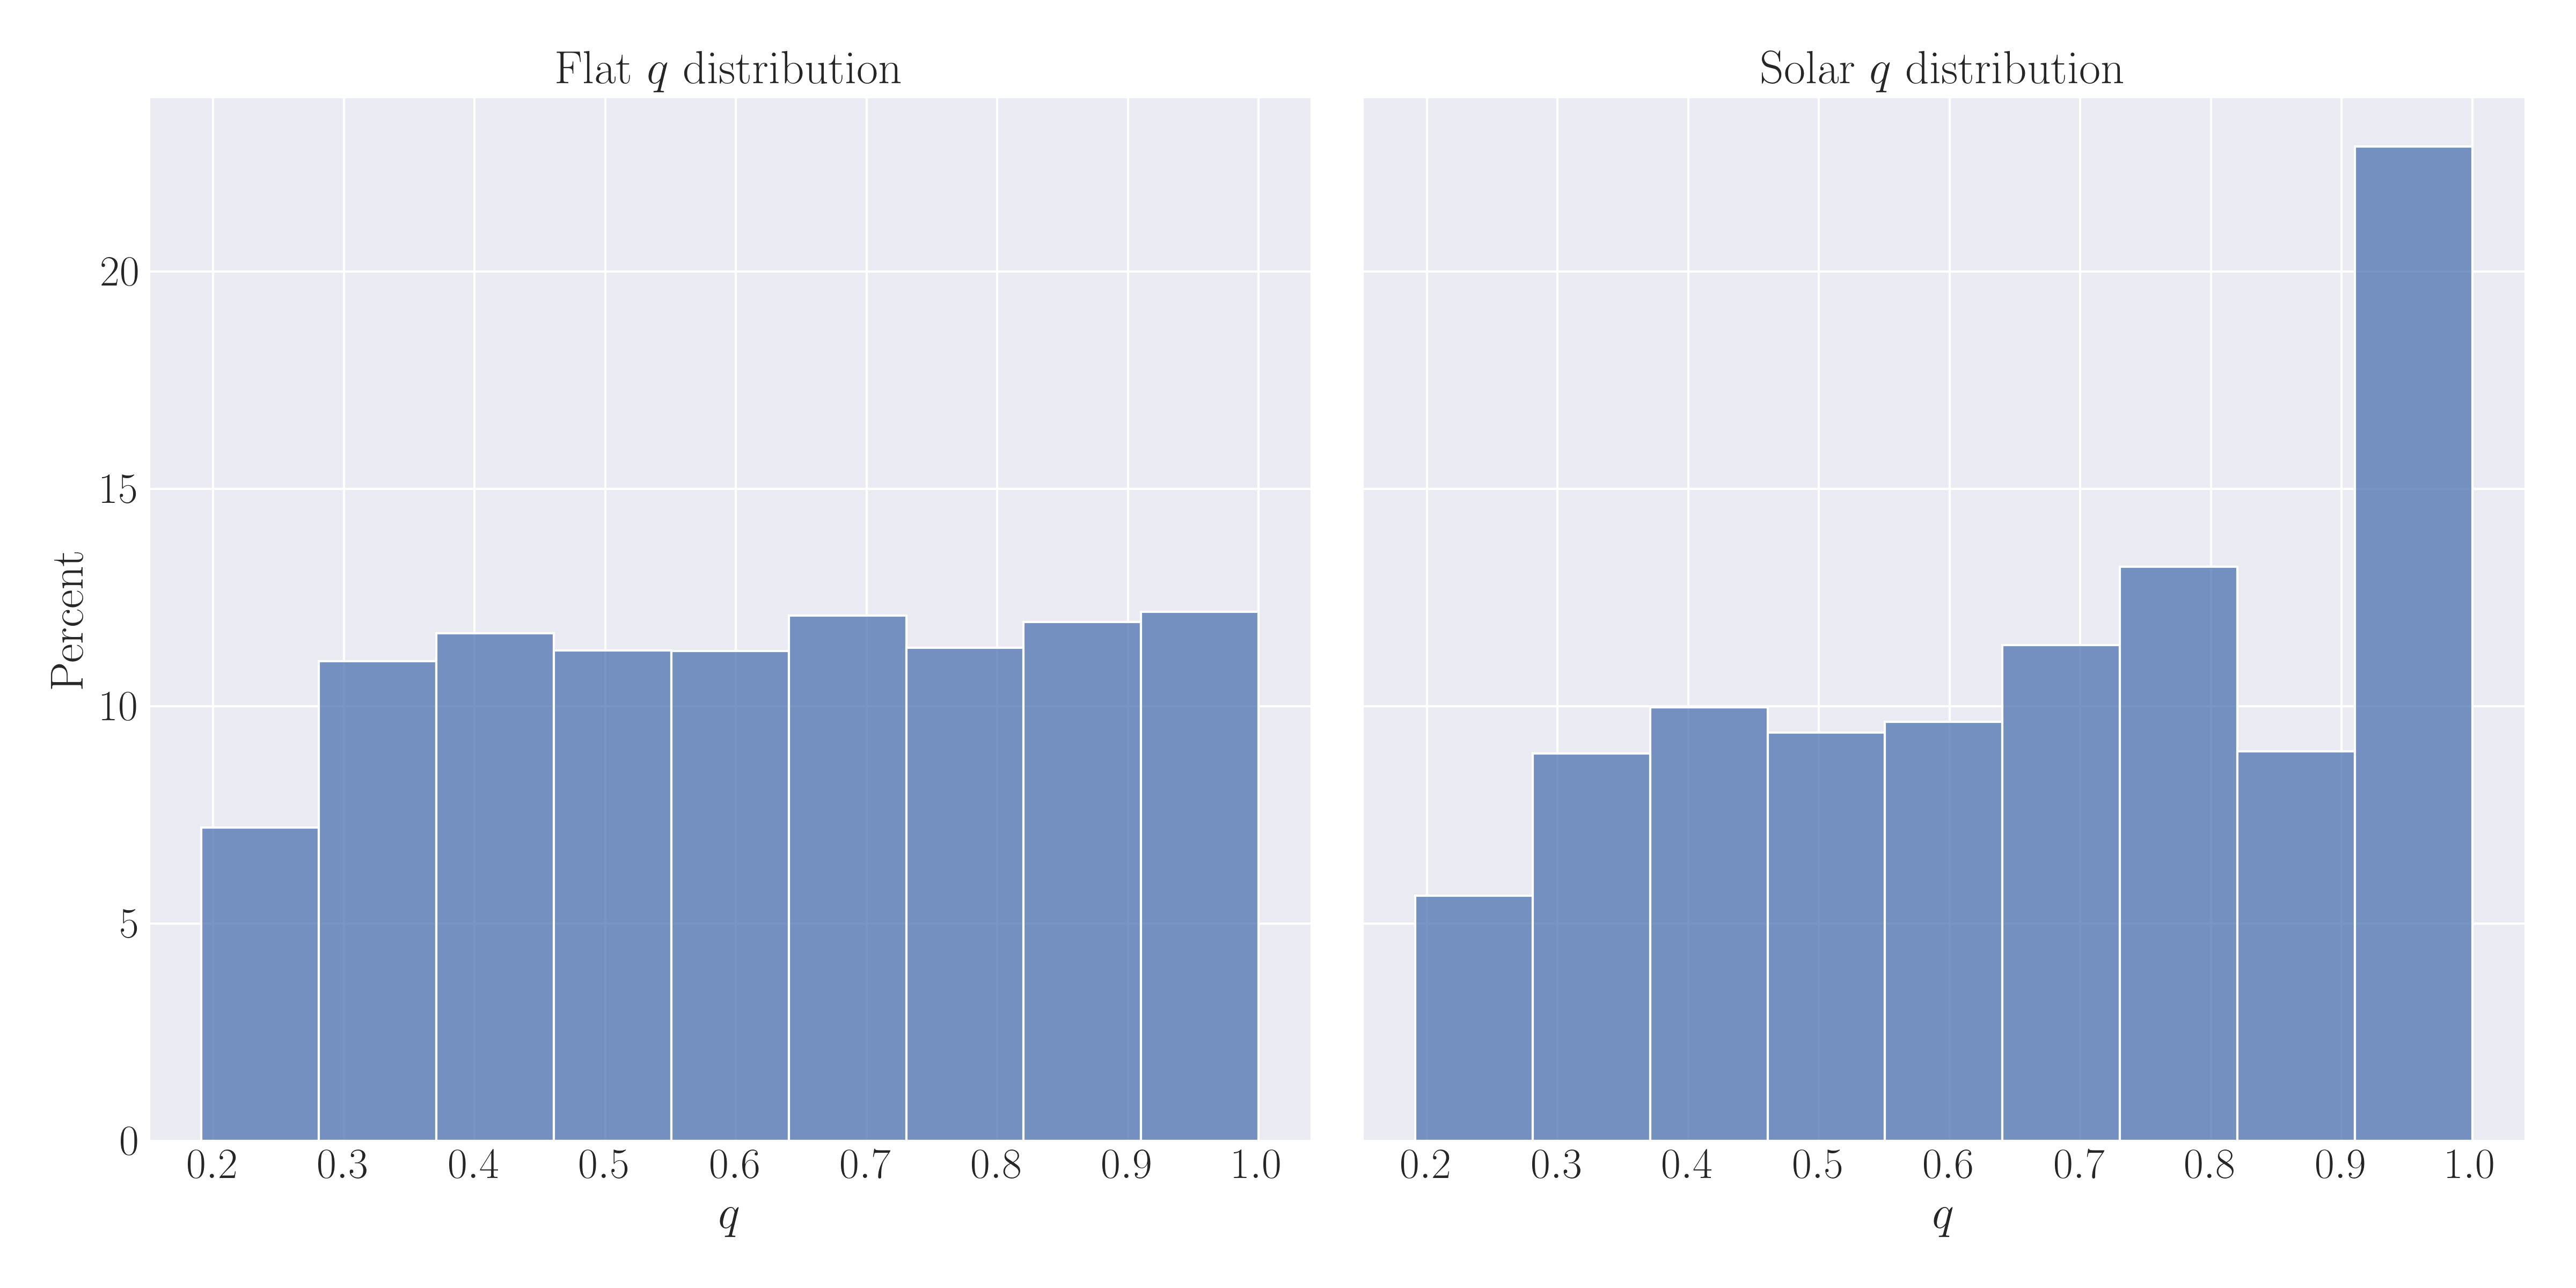
\includegraphics[width=\textwidth]{figures/q-dists.png}
    \caption{The resulting mass ratio distributions for the "flat" and "solar" mass ratio
        distributions. Both distributions are truncated and lowered at $q=0.2$ due to the relative
        lack low very low mass stars within the mass functions, making the creation of binary
        systems with a very low mass ratio impossible.}
    \label{fig:2/q-dists}
\end{figure}


After we have assigned a portion of the total binary fraction to each value of $q$, we then go
through each bin of main-sequence stars to make binaries. The companion mass for a given bin is
calculated for each value of $q$ in the mass ratio distribution and the number of binaries to make
is calculated using the portion of the binary fraction assigned to each value of $q$. After the
companion mass and number of binaries are set, we then remove mass from the primary bin and the bin
that most closely matches the mass of the companion and add the mass to a new bin with a mean mass
equal to the sum of the primary and companion masses. Through this process we move mass between bins
of differing \emph{mean} masses while conserving the \emph{total} mass in stars in the model.


We repeat this process for each bin of main-sequence stars until each bin has a binary fraction
equal to the total requested binary fraction and a mass ratio distribution identical to the
requested distribution, this results in the overall binary fraction and mass ratio distribution for
the cluster matching the requested values.


This process tends to create on the order of 150 new bins in our mass function which dramatically
increases the runtime of the \code{LIMEPY} models. In order to prevent this, we group together
binary bins of similar masses, forming 15 "binary bins" containing binary systems of similar total
mass but differing mass ratios. Figure \ref{fig:2/shifted-mf} shows the original main sequence bins,
plotted with the modified main sequence bins, binary bins and rebinned binary bins.


\begin{figure}
    \centering
    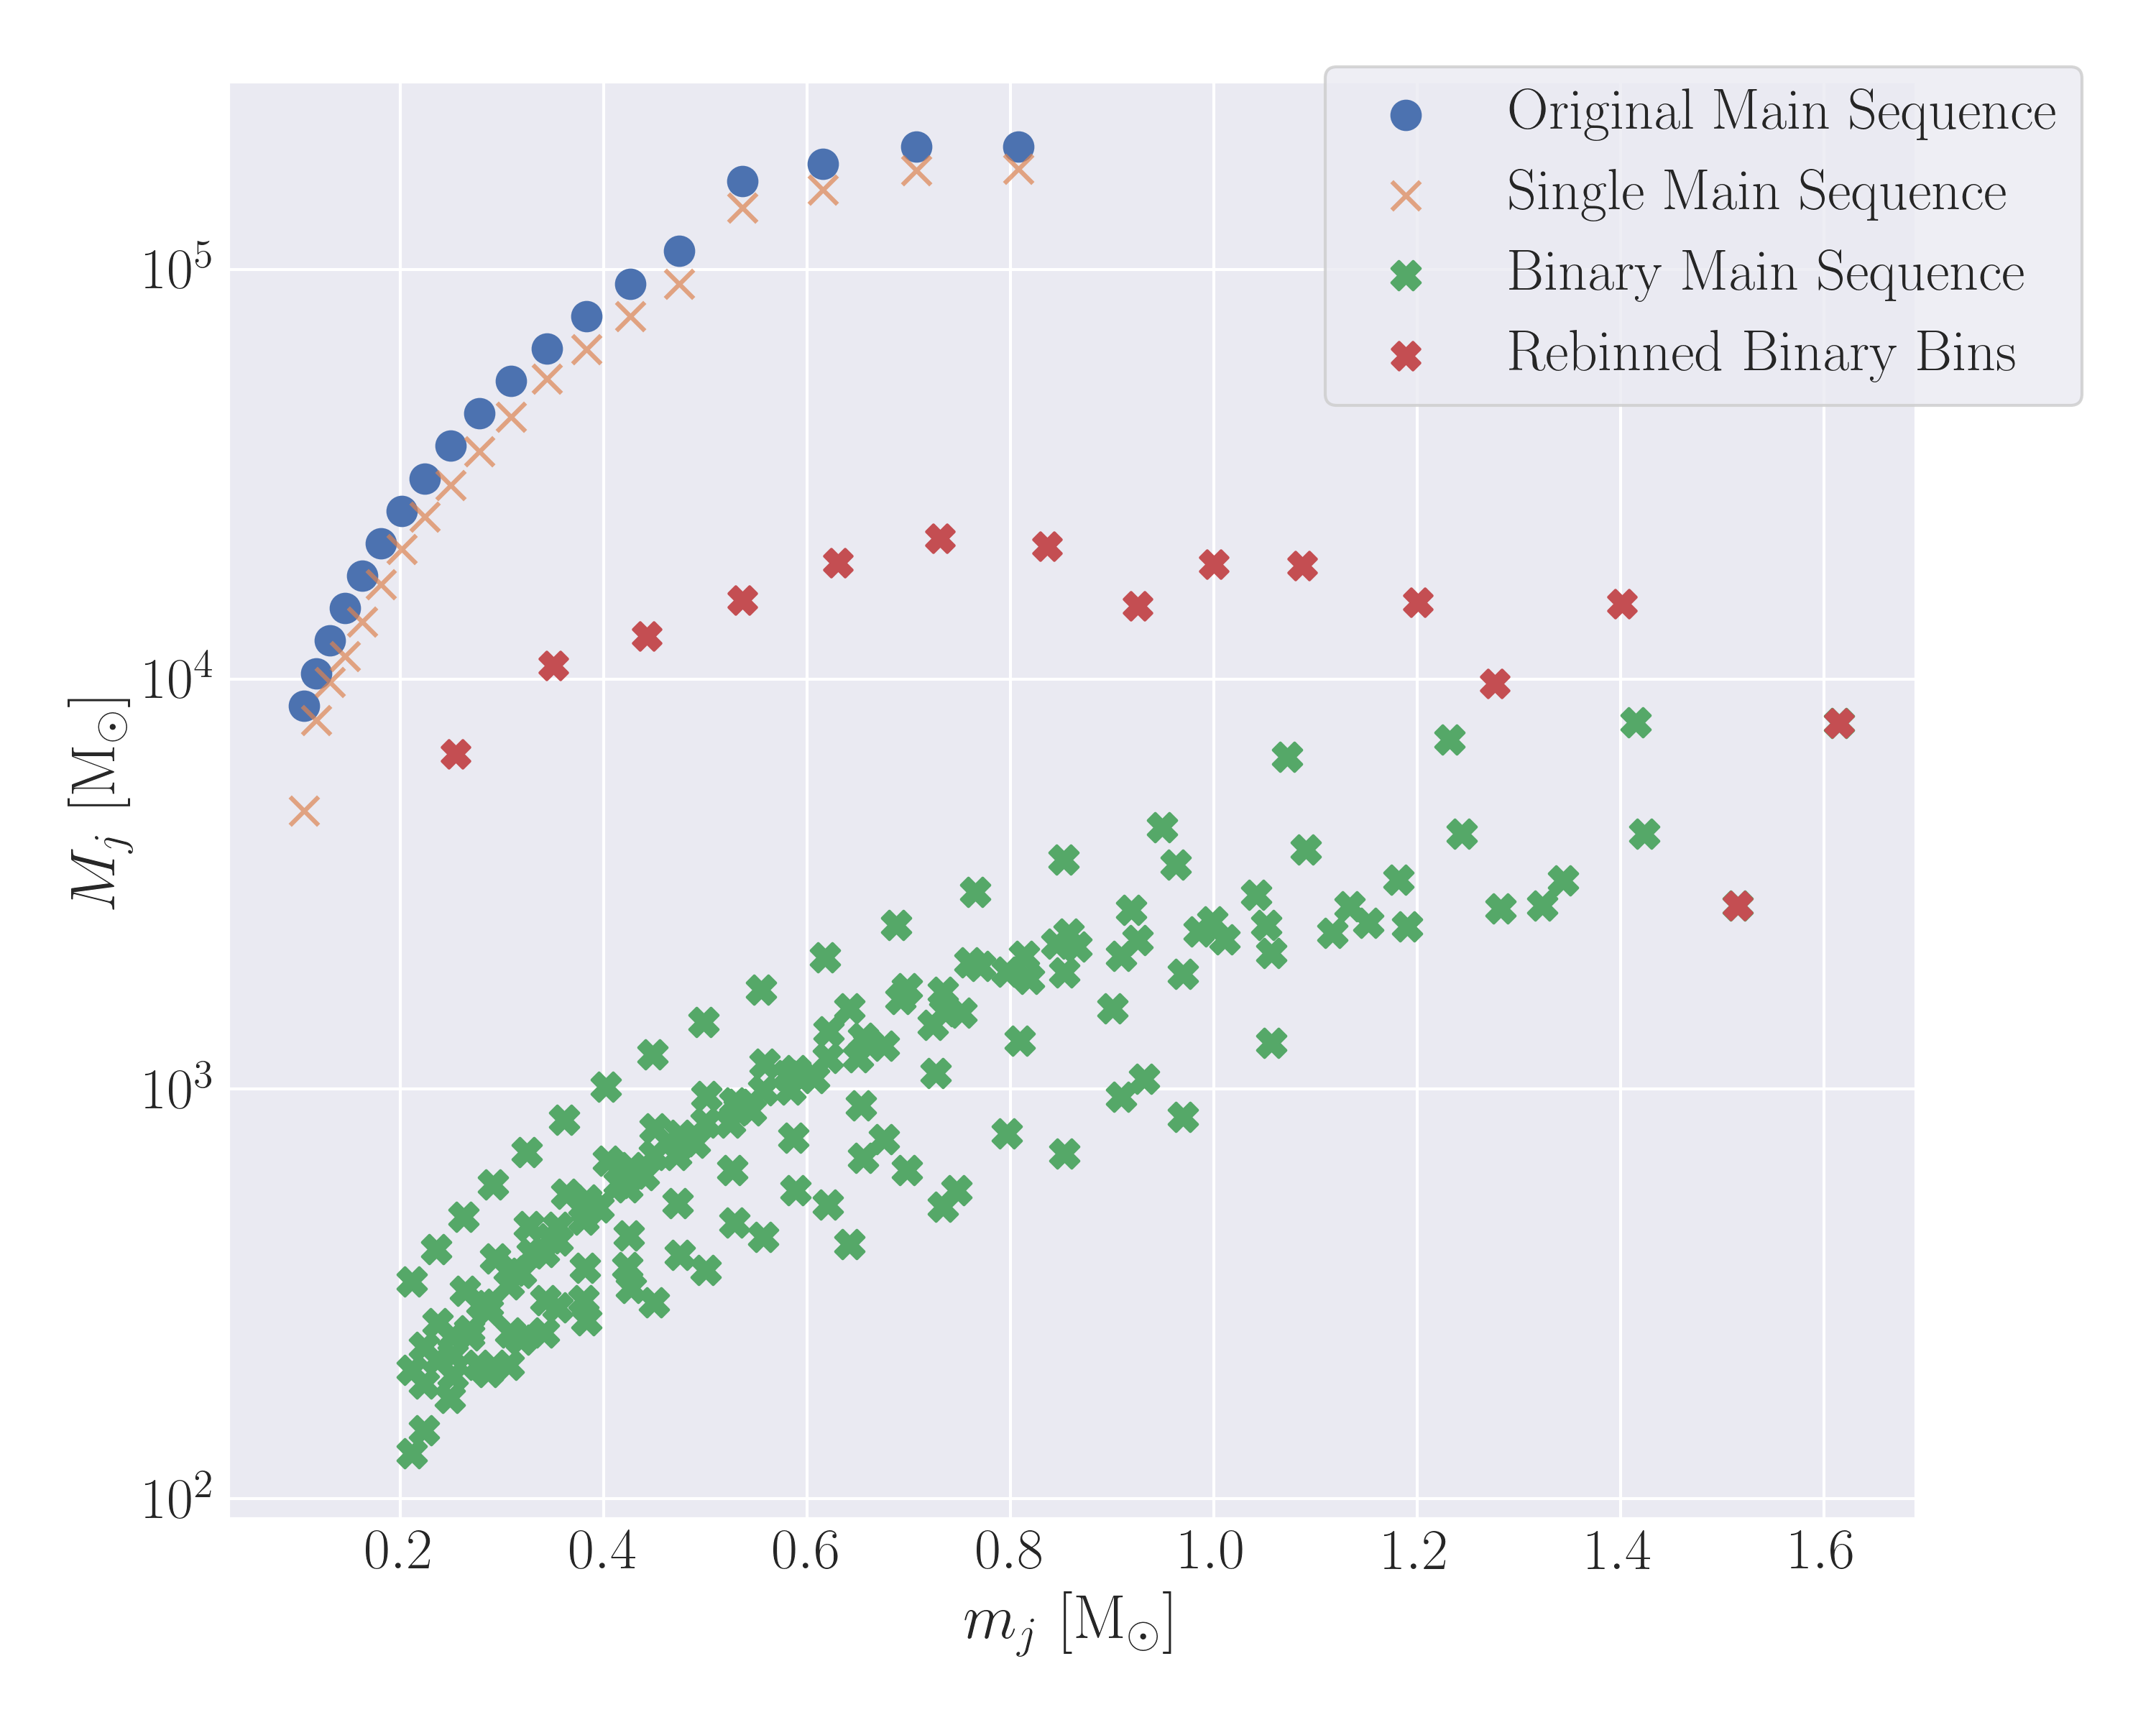
\includegraphics[width=0.8\textwidth]{figures/shifted-mf.png}
    \caption{The main-sequence portion of a mass function before and after binaries are added. $M_j$
        is the total mass within a bin while $m_j$ is the mean mass of the bin. The blue circles are
the original main sequence bins and the crosses are the modified main sequence bins. The
orange crosses show the single stars after mass has been removed to create binaries and the
many green crosses are the binary bins that are initially created. The red crosses are the
        rebinned binary bins which are actually used in the computation of the \code{LIMEPY}
        models.}
    \label{fig:2/shifted-mf}
\end{figure}



\section{Fitting Models to Data}


To fit our models to the data we use the \code{GCfit}
package\footnote{\url{www.github.com/nmdickson/gcfit}}. \code{GCfit} provides a uniform interface
for fitting \evolvemf{} and \code{LIMEPY} models to observations of clusters using either MCMC or
Nested Sampling.

For this project we use the MCMC backend which is powered by \code{emcee}
\citet{Foreman-Mackey2013,Foreman-Mackey2019}, an affine-invariant ensemble  sampler. We use 1024
walkers, initialized at a small randomized sphere around a reasonable initial guess  for the model
parameters. We run the chain for 2500 steps and discard the initial 2000 steps as the burn-in period
Trace and corner \citep{Foreman-Mackey2016} plots for all three chains are shown in Figures
\ref{fig:nobin_walkers} through \ref{fig:highbin_corner}.

\subsection{Likelihoods}

The majority of the likelihood functions we use are simple Gaussian likelihoods, provided below is
the likelihood for velocity dispersion profile data and all other likelihoods are of a similar form:

\begin{equation}
    \ln \left(\mathcal{L}\right)=\frac{1}{2}
    \sum_{r}\left(\frac{\left(\sigma_{\mathrm{obs}}(r)
        -\sigma_{\mathrm{model}}(r)\right)^{2}}{\delta \sigma_{\mathrm{obs}}^{2}(r)}
    -\ln \left(\delta \sigma_{\mathrm{obs}}^{2}(r)\right)\right)
\end{equation}

Where $\mathcal{L}$ is the likelihood, $\sigma$ is the line-of-sight velocity dispersion, $r$ is the
projected distance from the cluster centre, and $\delta \sigma$ is the uncertainty in the velocity
dispersion. The likelihoods for other observables are formulated in the same way, and the specifics
are discussed in \code{GCfit}'s documentation\footnote{\url{gcfit.readthedocs.io}}. The total
likelihood is therefore the sum of all the log-likelihoods for each set of observations.

For the mass function and number density profile likelihoods we include additional nuisance and scaling
terms.

In the case of the number density data we introduce a parameter $s^2$ which is added in quadrature
to the existing measurement uncertainties. This parameter allows us to add a constant amount of
uncertainty to all values in the data-set, effectively assigning less significance to the data
located furthest from the cluster centre where the number density is lowest. This allows us to
account for both background effects on the observations as well as for any effects that may be
present near the cluster boundary that the LIMEPY models do not account for such as the effects of
potential escapers (see \citealt{Claydon2019} for a discussion of potential escapers in equilibrium
models).

For the mass function data the only uncertainty included with the data is the Poisson counting
error. We introduce the nuisance parameter $F$ which is defined as a factor between 1 and 5 by which
we adjust each data point's absolute error. This error encapsulates additional sources of error that
may not have been accounted for as well as addresses the fact that the mass function is being
approximated as a broken power-law.


\subsubsection{Pulsar Likelihood}

As stated previously, the development of a method to use pulsar acceleration measurements to
constrain the models was performed as part of an earlier project, but we will provide a description
of the process below.




Pulsar period derivatives as measured by an observer are made up of several distinct components,
only one of which is related to the cluster potential. The effects of the proper motion of the
pulsar and the galactic potential of the pulsar are fairly easily constrained based on the pulsar's
position in the galaxy but, the effects of phenomena like magnetic breaking or accretion are not.
Equation \ref{eq:pular-components} shows the breakdown of the measured period derivative into
separate components where $(\dot{P}/P)_{int}$ is any change in period due to the effects intrinsic
to the pulsar like magnetic breaking or accretion, $a_c$ is the change due to the cluster's
gravitational potential and is the quantity we are interested in, $a_g$ is the effect of the
galaxy's gravitational potential and is easily adjusted for based on 47 Tuc's position within the
Milky Way, $a_s$ is the effect of the pulsar's proper motion and is similarly easy to compensate
for, $a_{DM}$ is the effect of the changing dispersion measure between the pulsar and the observer
and is a minor effect which we assume is well compensated for in our treatment of the intrinsic
period derivative.

\begin{equation}
    \left(\frac{\dot{P}}{P}\right)_{meas} = \left(\frac{\dot{P}}{P}\right)_{int} + \frac{a_c}{c} +
    \frac{a_g}{c} + \frac{a_s}{c} + \frac{a_{DM}}{c}
    \label{eq:pular-components}
\end{equation}



In order to constrain the 3D position of the pulsars within the cluster we adopt a model for the
internal gas distribution of the cluster from \citet{Abbate2018}. We adopt their best fitting model
which is a uniform distribution of ionized gas with a number density of $n = 0.23 \pm 0.05 \
    \text{cm}^{-3}$. We also adopt their estimate for the total dispersion measure between the observer
and the cluster centre: $DM_c = 24.38 \pm 0.02 \ \mathrm{pc \ cm}^{-3}$. By adopting a model for the
gas distribution, we are able to accurately determine the pulsars line-of-sight position ($l$)
within the cluster using the following equation (eq 28 in \citet{Abbate2018}):

\begin{equation}
    DM = n_g l + DM_c
    \label{eq:DM-los}
\end{equation}

Combining the accurate estimate of $l$ with the well-measured projected distance from the cluster
centre allows us to very accurately determine the pulsar's 3D position within the cluster.

In order to assign a likelihood to a particular $\dot{P}/P$ measurement we first use the
\texttt{LIMEPY} models to generate a line-of-sight acceleration profile for the given model. We then
use this acceleration profile to interpolate the possible line-of-sight positions for the pulsar.
These line-of-sight positions are then assigned a probability distribution based on a Gaussian
centred at the line-of-sight position as calculated from the DM with a dispersion equal to the
uncertainty of the DM-based line-of-sight position. The likelihood is the sum of the height of the
Gaussian at the interpolated line-of-sight positions from the model.


For pulsars that are not consistent with the uniform gas model (pulsars AA and D, see
\citealt{Abbate2018} for details) we instead assign a probability distribution to the line-of-sight
position based on the model density of pulsar-mass objects at the given line of sight. These
constraints are less precise than the DM-based constraints but allow us to use pulsars that are not
well-fit by a uniform gas distribution to constrain the properties of the cluster.

To constrain intrinsic spin-down of the pulsars, we assume the spin-down to be identical to pulsars
found in the galaxy, outside of clusters, and dependant only on their period. The field pulsars, as
they are unaffected by the cluster potential, can have their intrinsic spin-down determined
directly. A Gaussian kernel density estimator is computed in the field $P$-$\dot{P}$ space, which is
sliced along each cluster pulsar's period to extract a distribution of possible intrinsic values.
This distribution of intrinsic spin-down values is then convolved with the probability distribution
from the model.

A resulting probability distribution from this method is shown in Figure
\ref{fig:pulsar-likelihood}, while figures \ref{fig:pulsar_max_az} through \ref{fig:pulsar_Paz_spin}
show the agreement between best-fitting models and the period derivates for both orbital and spin
periods.

\begin{figure}
    \centering
    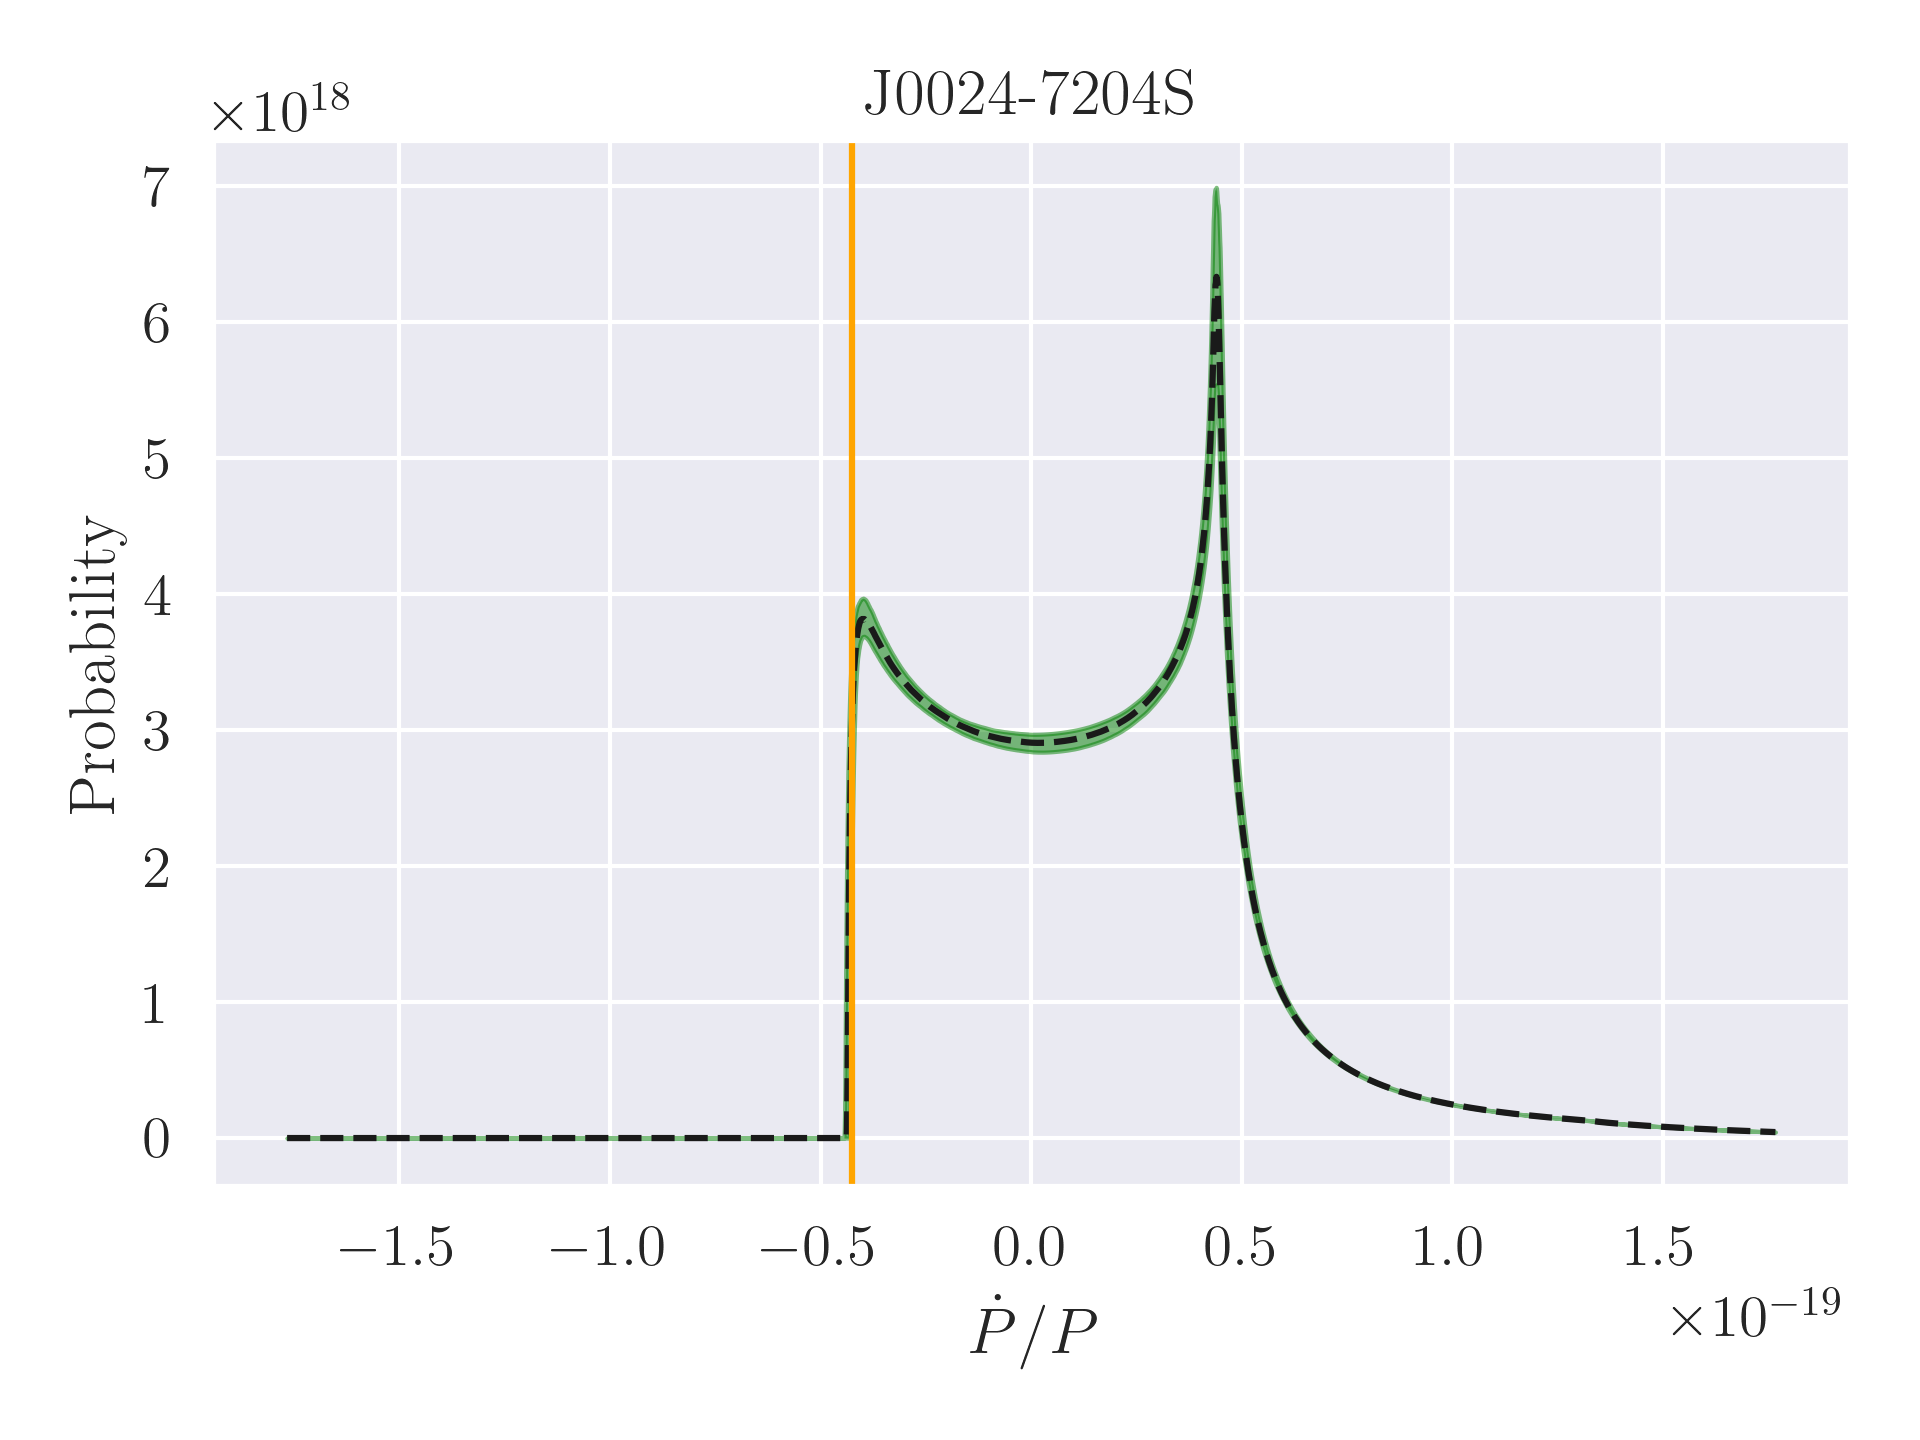
\includegraphics[width=0.8\textwidth]{figures/pulsar-likelihood.png}
    \caption{The resulting probability distribution for the spin period derivative of pulsar 47\,Tuc
        S from the method described above for the best-fitting models of 47\,Tuc. The green line is
        the likelihood of a given period derivative measurement given the best-fitting model
        parameters and the yellow line is the measured spin period derivative. The asymmetry in the
        distribution is due to the intrinsic spin-down of the pulsar, biasing the distribution to
        positive values of $\dot{P}/P$.}
    \label{fig:pulsar-likelihood}
\end{figure}

Many of the pulsars in 47\,Tuc are in binary systems and for 10 of these systems we have timing
solutions for the binary system. These binary periods are useful because they are on the order of
days rather than milliseconds. This means that the intrinsic effects that affect the spin periods
are negligible and any measured change in the period can be entirely attributed to the acceleration
from the cluster. Due to the much longer period, the number of detections is greatly reduced
resulting in a much larger uncertainty than the spin period derivatives, this large uncertainty
means the probability distributions based on orbital period derivatives have long tails and are not
suited for placing hard constraints on the mass distribution of the cluster, we nonetheless use the
orbital periods of these systems as an additional constraint on the cluster potential.


\subsection{Fitting Mass Functions to Observations}

When the mass function data was originally extracted, the mass was inferred based on the position of
the star on an isochrone fit to the cluster colour-magnitude diagram (see \citealt{Sollima2017} for
details). This means that any binary stars in the observed sample are interpreted as single stars
with a mass corresponding to a star with the combined colour of the two binary components and a
luminosity corresponding to the sum of the two components. When comparing our models to the data, we
want to extract the mass function profiles in the same way that the data was collected.

Additionally, when we move mass around to create binary bins in our models, we also affect the
surface density profiles which are used to compute the mass function profiles. In order to
compensate for these effects, we rescale the main-sequence surface density profiles to include the
stars which are in binary bins, according to the mass they would have been assigned using the
observational method described above, which assumed that all stars are single.

In order to determine the "observed" mass we use a grid of MIST isochrones
\citep{Dotter2016,Choi2016}\footnote{We use the \code{EZMIST} library to fetch and prepare the
isochrones. \code{EZMIST} is available online: \url{https://github.com/mfouesneau/ezmist}} computed
at a range of metallicities, at the age of the cluster. We use the isochrone closest to the model
parameters (an age of 11.75 Gyr, Fe/H of -0.75, and no stellar rotation) to determine the luminosity
of the binary components and then again use the isochrone to determine the observed mass of the
combined luminosities. Figure \ref{fig:2/isochrone} shows the derived relation between stellar mass
and luminosity used for these conversions. After having determined the mass that would have been
inferred for a binary system if it was assumed to be a single star, we then scale the surface
density profile of the main-sequence bin which most closely matches the "observed" mass of the
binary system by the total mass of the binary system which allows us to correct for both effects.


\begin{figure}
    \centering
    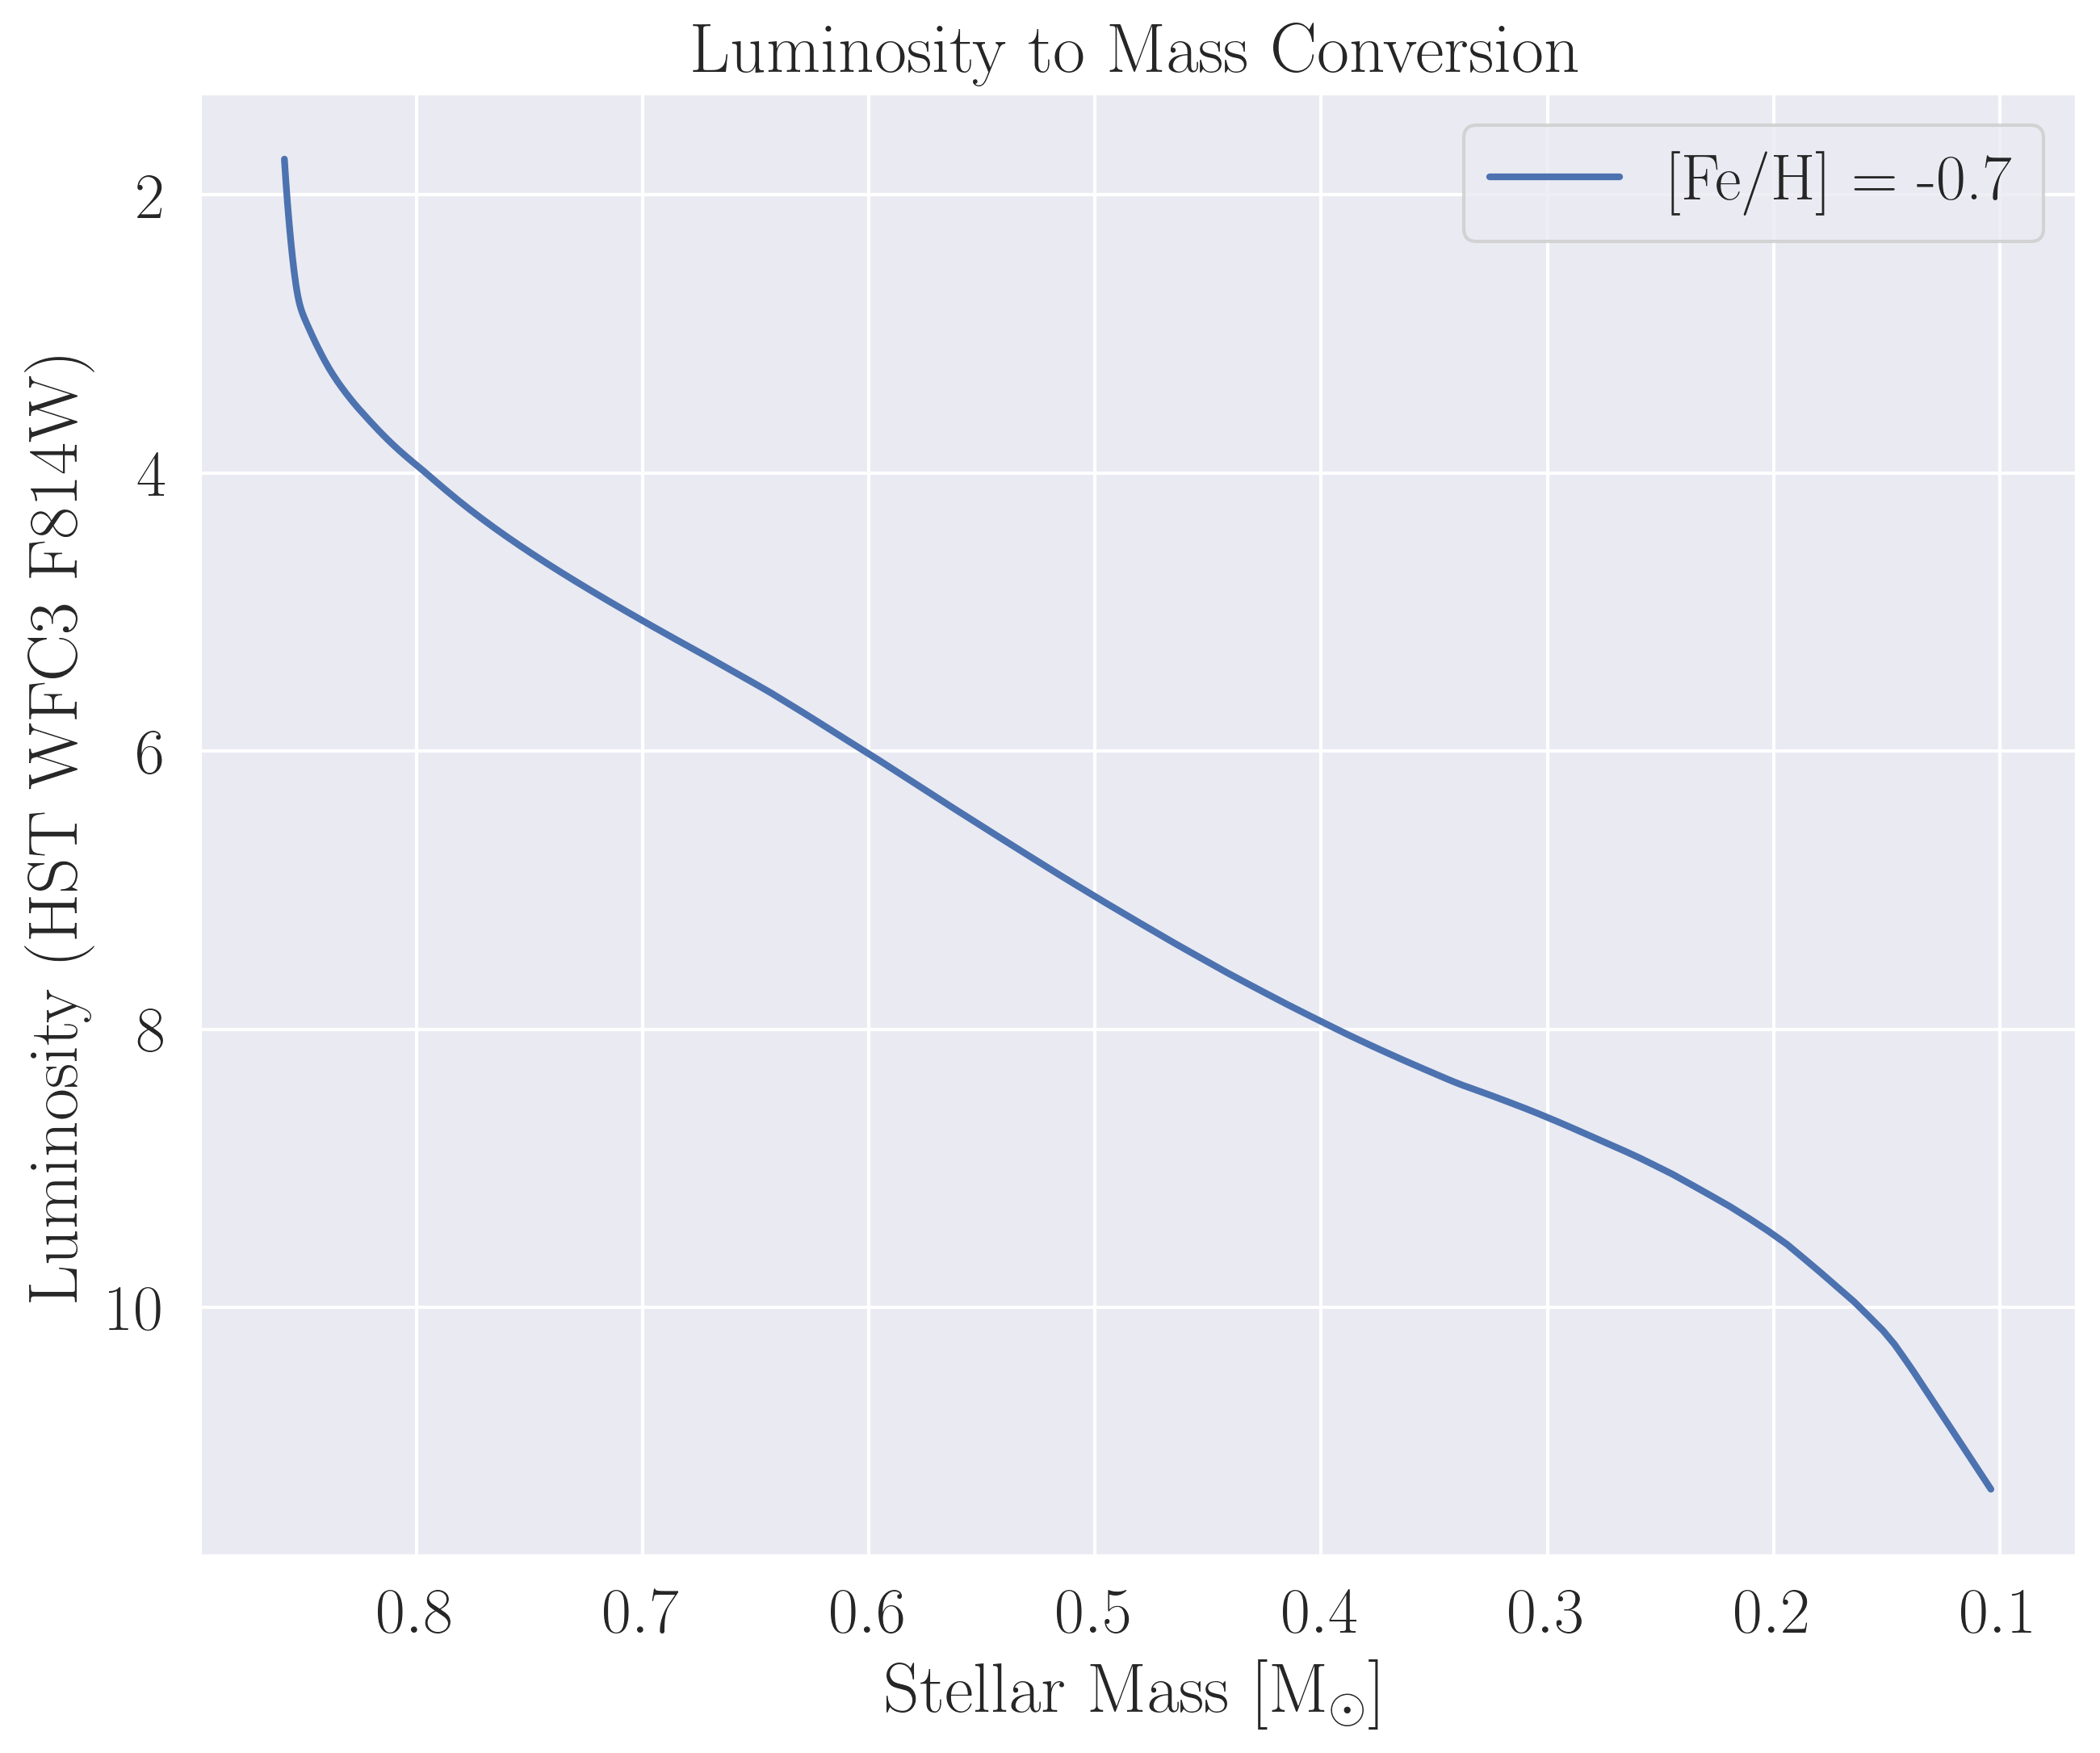
\includegraphics[width=0.8\textwidth]{figures/isochrone_conversion.png}
    \caption{Relation between stellar mass and luminosity through HST/WFC3's F814W filter, derived
        from a MIST isochrone. The F814W filter is used to replicate the original observations, see
        \citet{Sollima2017} for further details.}
    \label{fig:2/isochrone}
\end{figure}